
%\lcTex{%
%  \setlength{\BooleanSetOpsWidthRight}{1.4cm}
%  \setlength{\BooleanSetOpsWidthLeft}{\BooleanSetOpsWidthLineReal}
%  \addtolength{\BooleanSetOpsWidthLeft}{-\BooleanSetOpsWidthRight}
%  \begin{minipage}{\BooleanSetOpsWidthLeft}
%}
%
%\label{fig:simplePolygon}
%\begin{ccHtmlOnly}
%  <p><center>
%    <img src="./fig/simplePolygon.gif" border=0 alt="A simple polygon" align=right>
%  </center>
%\end{ccHtmlOnly}
%
%\label{fig:relativelySimplePolygon}
%\begin{ccHtmlOnly}
%  <p><center>
%    <img src="./fig/relativelySimplePolygon.gif" border=0 alt="A  relatively simple polygon" align=right>
%  </center>
%\end{ccHtmlOnly}
%
%\label{fig:notRelativelySimplePolygon}
%\begin{ccHtmlOnly}
%  <p><center>
%    <img src="./fig/notRelativelySimplePolygon.gif" border=0 alt="A polygon that is not simple or %relativelt simple" align=right>
%%  </center>
%%\end{ccHtmlOnly}

\section{Terms and Definitions\label{bso_sec:bso_def}}
% =================================================

\begin{figure}[!htp]
\begin{center}
\begin{ccTexOnly}
  \begin{center}
  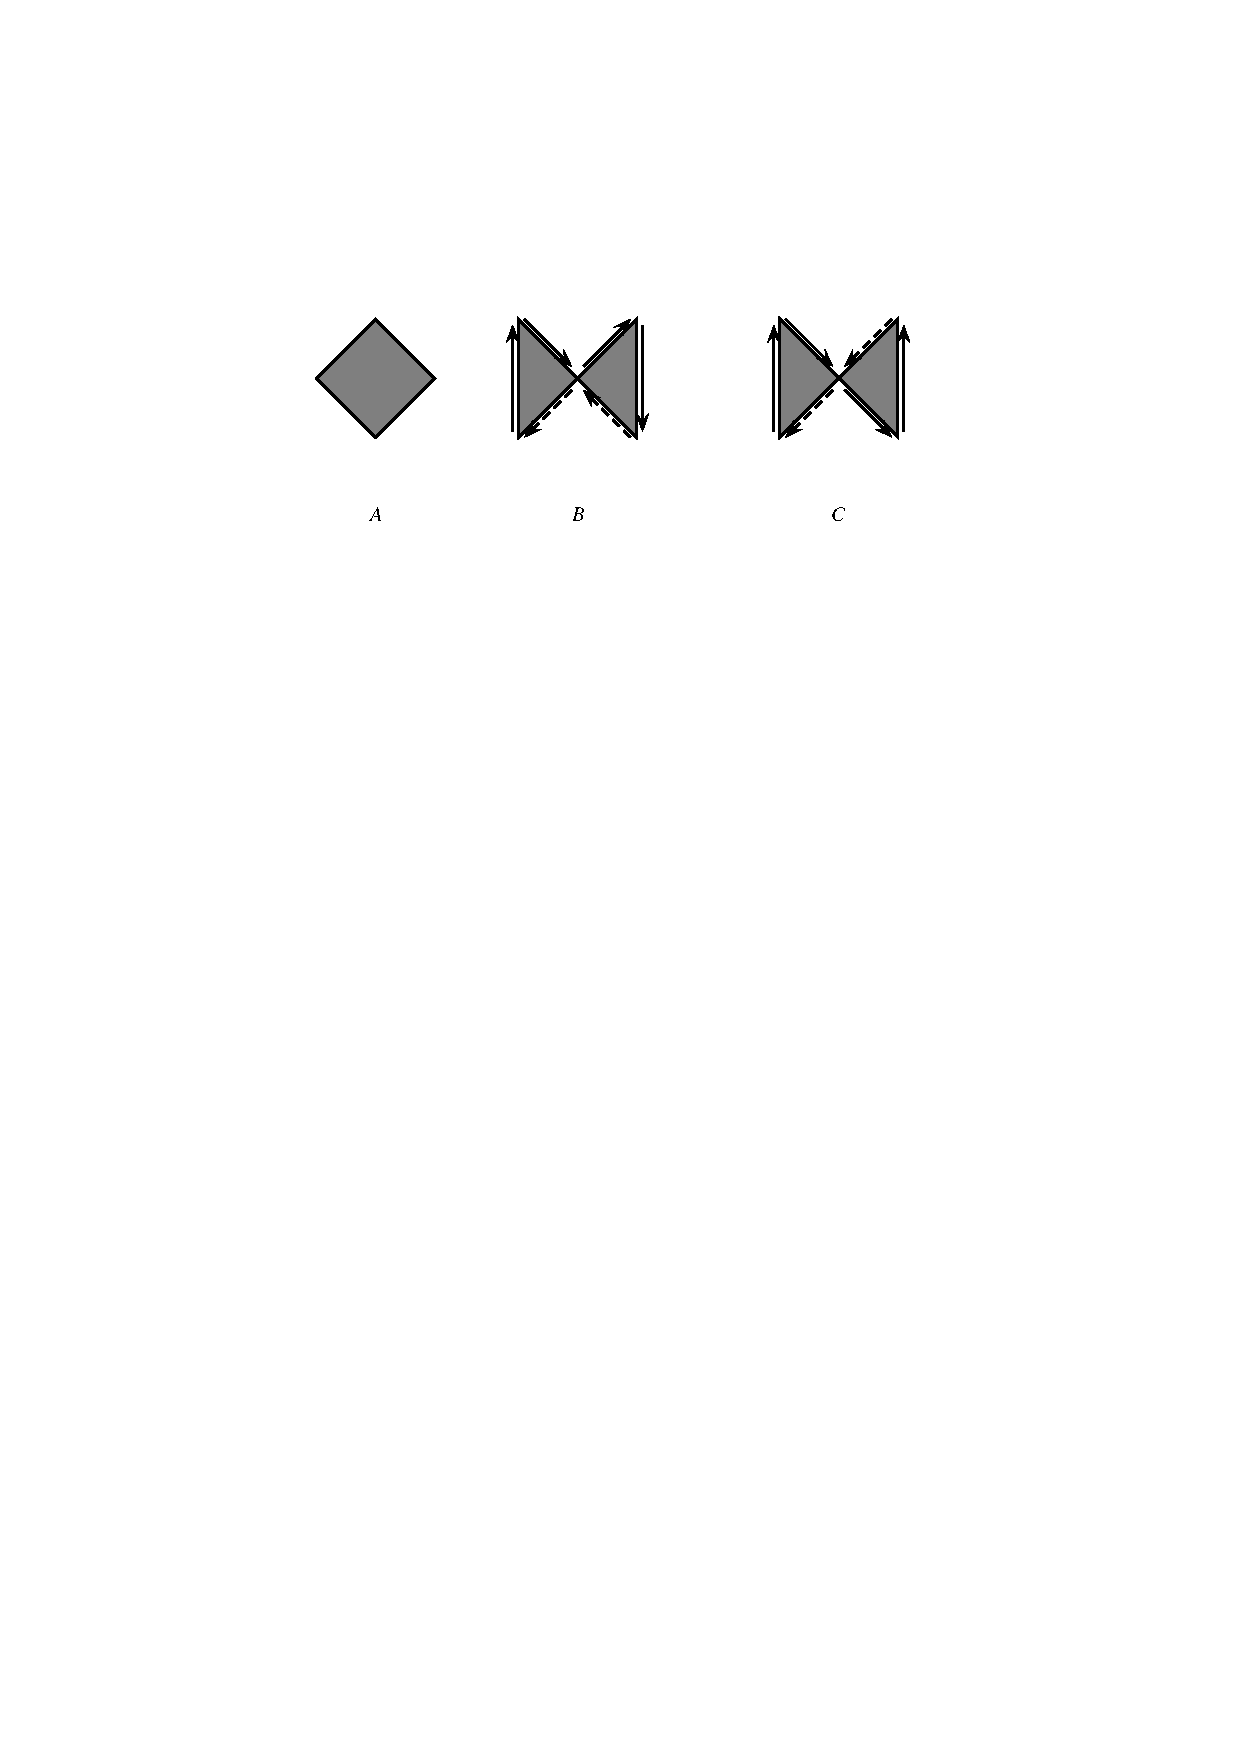
\includegraphics{Boolean_set_operations_2/fig/simpleDefsExamples}
  \end{center}
\end{ccTexOnly}
\label{fig:simpleDefsExamples}
\begin{ccHtmlOnly}
  <p><center>
    <img src="./fig/simpleDefsExamples.gif" border=0 alt="Example Polygons">
  </center>
\end{ccHtmlOnly}
\caption{Examples of polygons. (a)~A simple polygon. (b)~A relatively simple polygon (c)~A polygon that is neither simple nor relatively simple} 
\end{center}
\end{figure}
\begin{itemize}

\item The counterclockwise cyclic sequence of alternating polygon edges and
polygon vertices is referred to as the polygon \textbf{(outer) boundary}.

\item A polygon whose curves are pairwise disjoint in their interior, and whose vertices' degree equals two is defined as a \textbf{Simple polygon}. Such a polygon has a well-defined interior and exterior and is topologically equivalent to a disk.  Note that while traversing the edges of the relatively simple polygon illustrated above (B), no curve is crossed over.

\item A \textbf{Relatively simple} polygon allows vertices with a degree$>$2, but all of its edges are disjoint in their interior. Furthermore, it must be an orientable polygon.  Namely when it is inserted into an arrangement and its outer boundary is traversed, the same face is adjacent to all of the halfedges (no crossing over any curve during the traversal).  
%\textbf{insert relativelySimplePolygon.tex}\\
Note that while polygon C has the same curves as polygon B, traversal of the curves leads to crossing over a previously traversed curve, and is therefore neither simple nor relatively simple.  
%\textbf{insert NotRelativelySimplePolygon.tex}\\ \\

\item A polygon in our context must be relatively simple and its outer boundary vertices must be ordered in a counterclockwise direction around the interior of the polygon.
We extend the notion of a polygon to a \textbf{point set} in $\real^2$
that has  a topology of a polygon and its boundary edges must map to
$x$-monotone curves, and refer to it as a \textbf{general polygon}. We
sometimes use the term {\em polygon} instead of general polygon for
simplicity hereafter.

\item A \textbf{polygon with holes} represents a point set that may
be bounded or unbounded. In case of a bounded set, its {\em outer
boundary} is represented as a {\em relatively simple } (but not necessarily simple) polygon, whose vertices are oriented in a {\em counterclockwise }
order around the interior of the set. In addition, the set may contain
{\em holes}, where each hole is represented as a {\em simple}
polygon, whose vertices are oriented in a {\em clockwise} order around the
interior of the hole. Note that an unbounded polygon without holes
spans the entire plane. Vertices of holes may coincide with vertices
of the boundary.

\item A \textbf{regularized Boolean set-operation} $\mbox{op}^*$ can be obtained by
first taking the interior of the resultant point set of an {\em ordinary}
Boolean set-operation $(P\ \mbox{op}\ Q)$ and then by taking the
closure~\cite{cgal:h-sm-04}. That is,
$P\ \mbox{op}^*\ Q = \mbox{closure}(\mbox{interior} (P\ \mbox{op}\ Q))$.
Regularized Boolean set-operations appear in Constructive Solid
Geometry (CSG), because regular sets are closed under regularized
Boolean set-operations, and because regularization eliminates lower
dimensional features, namely isolated vertices and antennas, thus
simplifying and restricting the representation to physically meaningful
solids. Our package provides regularized operations on polygons and
general polygons, where the edges of a general polygon may be
general $x$-monotone curves, rather than being simple line segments.
% see below for an example (unique.tex?). 
\end{itemize}
% ----------------------------------
\subsection{Conditions for Valid Polygons\label{bso_ssec:polygon_validation}}
% ----------------------------------

In our context, a polygon must uphold the following conditions:\\
\begin{enumerate}
 \item\textit{Closed Boundary} - the polygon's outer boundary must be a connected sequence of curves, that start and end at the same vertex.
\item \textit{Simplicity} - the polygon must be simple.
\item \textit{Orientation} - the polygon's outer boundary must be \textit{counter-clockwise oriented}.
\end{enumerate}
 

% ----------------------------------
\subsection{Conditions for Valid Polygons with Holes \label{bso_ssec:polygon_with_holes_validation}}
% ----------------------------------
In our context, a polygon with holes must uphold the following conditions:\\
\begin{enumerate}
\item \textit{Closed Boundary} - both the outer boundary and the holes must be closed polygons as defined above.
\item \textit{Simplicity} - the outer boundary must be a \textit{\textbf{relatively} simple} polygon (as defined above). Every hole must be a \textit{simple} polygon. 
\item \textit{Orientation} - The polygon with holes must have an outer boundary with  \textit{counter clockwise orientation}. Every hole's outer boundary should have  \textit{clockwise orientation}. 
\item \textit{The holes and the outer boundary must be pairwise disjoint,except maybe on vertices}. 
\begin{itemize}
\item \textit{All holes are contained in the outer boundary} - holes must be contained inside the outer boundary and must be disjoint from it (except on vertices). 
\item \textit{Pairwise disjoint holes (on interior)} - the polygon's holes must be \textit{pairwise disjoint}, except for intersection on a joint vertex/vertices. 

\end{itemize}
\end{enumerate}


